\documentclass[12pt]{article}
\usepackage{config}

%O preenchimento desses dados atesta que essa avaliação foi produzida de forma totalmente individual por parte do discente. O mesmo tem ciência que a identificação de respostas copiadas será levada para a coordenação e a direção do curso tomarem as medidas cabíveis.
\aluno{\textcolor{red}{EXPECTATIVA DE RESPOSTAS}%Escreva o seu nome completo aqui
}
\matricula{%Escreva a sua matrícula aqui
}

% Coloque pacotes adicionais aqui, se for necessário

%Para anexar alguma imagem, basta deixar o arquivo na pasta "imagens" e usar o comando abaixo:
%\imagem[width=7cm]{NOME DO ARQUIVO COM EXTENSÃO}{LEGENDA DA FIGURA} % Lembrar do "../"

\begin{document}
   \maketitle
   A avaliação a seguir deve ser feita usando os conhecimentos estudados na Unidade 1 da disciplina.

 %--------------------------------------------------  
 % QUESTÕES DE CONJUNTOS
 %--------------------------------------------------
   
   \begin{enumerate}
        \item \emph{(3{,}0 pontos)} Sejam $A$, $B$ conjuntos quaisquer. Classifique como verdadeira ou falsa a sentença $$(A \cup B)^C \subseteq A^C.$$ Justifique com propriedades do nosso material no caso de ser verdadeira ou dê um contra-exemplo no caso da sentença ser falsa.
            \begin{proof} 
                % Escreva aqui a solução da questão 1.
\textbf{VERDADEIRA}

\textcolor{red}{ VERSÃO 1 } %Letícia

%\textbf{VERDADEIRA}

De uma das propriedades da união de conjuntos, sabemos: $A \subseteq (A \cup B)$.

Das propriedades de complementar de um conjunto, sabemos: $X \subseteq Y \implies Y^C \subseteq X^C$.

Aplicando essa propriedade à primeira inclusão acima:

$A \subseteq (A \cup B) \implies (A \cup B)^{C} \subseteq A^{C}$.
Portanto, a sentença é verdadeira.

\bigskip

\textcolor{red}{CHAVE DE PONTUAÇÃO:
\begin{itemize}
    \item  Inclusão pela união \emph{(1,5 ponto)};
    \item  Inclusão pela propriedade de complementar \emph{(1,5 ponto)}.
\end{itemize} }


\bigskip


\textcolor{red}{ VERSÃO 2} %Esther



Perceba que, por De Morgan, $(A \cup B)^C = A^C\cap B^C$ e, em particular, $(A \cup B)^C \subseteq A^C\cap B^C$. Por propriedade de interseção, $A^C\cap B^C\subseteq A^C$. Logo, por transitividade, $(A \cup B)^C \subseteq A^C.$


\bigskip


%\textcolor{red}{ VERSÃO 3} % autor




%\bigskip







\textcolor{red}{CHAVE DE PONTUAÇÃO:
\begin{itemize}
    \item  Inclusão pelo DeMorgan \emph{(1,0 ponto)};
    \item  Inclusão pela interseção \emph{(1,0 ponto)};
    \item  Inclusão pela transitividade \emph{(1,0 ponto)}.
\end{itemize} } % Lembrar do "../"
           \end{proof}
        \item \emph{(3{,}0 pontos)}  Sejam $A$, $B$ conjuntos quaisquer. Classifique como verdadeira ou falsa a sentença $$B \subseteq (A \setminus B)^C.$$ Justifique com propriedades do nosso material no caso de ser verdadeira ou dê um contra-exemplo no caso da sentença ser falsa.
            \begin{proof} 
                    % Escreva aqui a solução da questão 2.
\textbf{VERDADEIRA}

\textcolor{red}{ VERSÃO 1 } %Letícia

De uma das propriedades da interseção de conjuntos, temos que $A \cap B^{C} \subseteq B^{C}$.
Então, podemos reescrever:
\begin{align*}
    A \cap B^{C} \subseteq B^{C} &\implies (B^{C})^{C} \subseteq (A \cap B^{C})^{C} \tag{$X \subseteq Y \implies Y^C \subseteq X^C$} \\ 
    & \implies B \subseteq (A \cap B^{C})^{C} \tag{$(X^C)^C = X$}\\ 
    &\implies B \subseteq (A \setminus B)^{C} . \tag{$X\setminus Y  = X \cap Y^{C}$}
\end{align*}

Logo, a relação de inclusão é verdadeira.




\bigskip

\textcolor{red}{CHAVE DE PONTUAÇÃO:
\begin{itemize}
    \item  Inclusão pela interseção \emph{(1,0 ponto)};
    \item Uso de $X \subseteq Y \implies Y^C \subseteq X^C$ e do complementar do complementar\emph{(1,0 ponto)};
    \item  Uso da igualdade $X \setminus Y = X \cap Y^C$ \emph{(1,0 ponto)}.
\end{itemize} } 

\bigskip


\textcolor{red}{ VERSÃO 2} %Letícia


Analisando o conjunto do lado direito da relação de inclusão, perceba que a diferença entre os conjuntos pode ser reescrita como a interseção do conjunto à esquerda da diferença ($A$) e do complementar do conjunto à direita ($B$), logo 
\begin{align}
    (A\setminus B)^{C} & = (A \cap B^{C})^{C} & \tag{diferença de conjuntos} \\
    & = A^{C} \cup B. & \tag{De Morgan e $(X^C)^C = X$}
\end{align}

Então,  $B \subseteq (A \setminus B)^{C}$ é equivalente a $B \subseteq A^{C} \cup B$. De uma das propriedades da união de conjuntos, sabe-se que essa relação de inclusão é verdadeira.



\bigskip

%\textcolor{red}{ VERSÃO 3} % autor




%\bigskip

\textcolor{red}{CHAVE DE PONTUAÇÃO:
\begin{itemize}
    \item  Inclusão pela união \emph{(1,0 ponto)};
    \item  Igualdade (ou inclusão) pelo DeMorgan e o complementar do complementar\emph{(1,0 ponto)};
    \item  Uso da igualdade $X \setminus Y = X \cap Y^C$ \emph{(1,0 ponto)}.
\end{itemize} } % Lembrar do "../"
           \end{proof}
           \item \emph{(3{,}0 pontos)} Sejam $A$, $B$ conjuntos quaisquer. Classifique como verdadeira ou falsa a sentença $$\mathcal U \setminus A \subseteq (A \cap B)^C.$$ Justifique com propriedades do nosso material no caso de ser verdadeira ou dê um contra-exemplo no caso da sentença ser falsa.
           \begin{proof} 
                % Escreva aqui a solução da questão 3.
\textbf{VERDADEIRA}

\textcolor{red}{ VERSÃO 1 } %Letícia

%\begin{enumerate}[label=\Roman*)]
%    \item Observe que a diferença entre os conjuntos pode ser reescrita como:
    
%    $\mathcal{U} \setminus A = \mathcal{U} \cap A^{C} = A^{C}$. Pela definição de igualdade de conjuntos, $(\mathcal{U} \setminus A) \subseteq A^{C}$.

%    \item De uma das propriedades da interseção de conjuntos: $(A \cap B) \subseteq A$. 
%    De uma das propriedades do complementar, $(A \cap B) \subseteq A \implies A^{C} \subseteq (A \cap B)^{C}$.

%    Por transitividade, de (I) temos que: $(\mathcal{U} \setminus A) \subseteq (A \cap B)^{C}$. Portanto, a relação de inclusão é verdadeira.
 
%\end{enumerate}
De uma das propriedades da interseção de conjuntos, temos que $(A \cap B) \subseteq A$.
Então, podemos reescrever:
  \begin{align*}
      (A \cap B) \subseteq A &\implies A^{C} \subseteq (A \cap B)^{C} \tag{$X \subseteq Y \implies Y^C \subseteq X^C$} \\
      &\implies (\mathcal{U} \setminus A) \subseteq (A \cap B)^{C}. \tag{$\mathcal{U} \setminus X= X^{C}$}
  \end{align*}

\bigskip

\textcolor{red}{CHAVE DE PONTUAÇÃO:
\begin{itemize}
    \item  Inclusão pela interseção \emph{(1,0 ponto)};
    \item Uso de $X \subseteq Y \implies Y^C \subseteq X^C$ \emph{(1,0 ponto)};
    \item  Uso da igualdade $\mathcal{U} \setminus X= X^{C}$ \emph{(1,0 ponto)}.
\end{itemize} } 

\bigskip




\textcolor{red}{ VERSÃO 2 } %Letícia

Observando o conjunto do lado esquerdo da relação de inclusão, percebe-se que a diferença entre os conjuntos pode ser reescrita como a interseção do conjunto à direita da diferença ($\mathcal{U}$) e do complementar do conjunto à esquerda ($A$). Ou de forma mais direta, a diferença entre o universo e o conjunto $A$ é igual ao complementar de $A$.

\begin{align*}
    \mathcal{U} \setminus A & = \mathcal{U} \cap A^{C} \\
    & = A^{C}.
\end{align*}

No lado esquerdo da inclusão, por De Morgan, temos:
$$(A \cap B)^{C} = A^{C} \cup B^{C}.$$

Então,  $ \mathcal{U} \setminus A \subseteq (A \cap B)^{C}$ é equivalente a $A^{C} \subseteq A^{C} \cup B^{C}$. De uma das propriedades da união, a sentença é verdadeira.

\bigskip



%\textcolor{red}{ VERSÃO 3} %autor





\bigskip

\textcolor{red}{CHAVE DE PONTUAÇÃO:
\begin{itemize}
    \item  Uso da igualdade $\mathcal{U} \setminus X= X^{C}$ \emph{(1,0 ponto)};
    \item  Igualdade pelo De Morgan \emph{(1,0 ponto)};
    \item  Inclusão pela união \emph{(1,0 ponto)}.
\end{itemize} } % Lembrar do "../"
           \end{proof}

%--------------------------------------------------  
 % QUESTÕES DE EQUAÇÕES E INEQUAÇÕES
 %--------------------------------------------------
       \item \emph{(3{,}0 pontos)} Diofanto de Alexandria (século III d.C.) foi um importante matemático e em sua lápide há o seguinte problema:
       
       ``Deus lhe concedeu a sexta parte da vida para ser menino; e uma duodécima parte a mais para que os seus pêlos começassem a crescer. Depois de uma sétima parte adicional, ele se casou. Passados cinco anos, nasceu seu filho. Mas o destino decidiu que o filho viveria apenas metade do tempo de vida total do pai. Após a morte do filho, Diofanto viveu ainda quatro anos, aliviando sua dor com o estudo dos números.'' 
       
       Sabendo que uma duodécima parte é uma divisão por doze avos, quantos anos viveu Diofanto?  
        \begin{solution} 
                % Escreva aqui a solução da questão 4.


\textcolor{red}{ VERSÃO 1 } %ian

Seja $V$ a quantidade de anos vivida por Diofanto. Analisando o texto, as partes da vida de Diofanto indicadas são as seguintes:

``Deus lhe concedeu a \textbf{sexta parte \emph{da vida}} para ser menino'' : $\dfrac{V}{6}$.

``e uma \textbf{duodécima parte \emph{a mais}} para que os seus pêlos começassem a crescer'': $\dfrac{V}{12}$.

``Depois de uma \textbf{sétima parte \emph{adicional}}, ele se casou'': $\dfrac{V}{7}$.

``\textbf{\emph{Passados} cinco anos}, nasceu seu filho'': $+5$ anos. 

``Mas o destino decidiu que \textbf{o filho} viveria apenas \textbf{metade do tempo de \emph{vida total do pai}}'': $\dfrac{V}{2}$.

``\textbf{\emph{Após} a morte do filho}, Diofanto \textbf{viveu \emph{ainda} quatro anos}'': $+4$ anos.

%A análise consiste em perceber que: os períodos se referem sempre ao \textbf{todo} de sua vida; os períodos nunca se referem a anos "restantes"; os períodos são distintos, sem sobreposição de intervalo de tempo; os períodos narrados juntos compreendem \textbf{toda} a sua vida; a informação numérica do nascimento e morte do seu filho permite determinar numericamente quantos anos teve de vida. Fazemos essa determinação pela equação:

Disso, segue a solução da equação:

\begin{align*}
    \dfrac{V}{6} + \dfrac{V}{12} + \dfrac{V}{7} + 5 + \dfrac{V}{2} + 4 = V &\iff \dfrac{14V+7V+12V+42V}{84} + 9 = V\\
    &\iff \dfrac{14V+7V+12V+42V}{84} + 9 = V\\
    &\iff 9 = V - \dfrac{75V}{84}\\
    &\iff 9 = \dfrac{9V}{84}\\
    &\iff V = 84.
\end{align*}

Portanto, Diofanto viveu 84 anos.

\textcolor{red}{ VERSÃO 2 } %Esther

Seja a quantidade de anos vividas por Diofanto denotada por $x$. Do texto, tiramos as seguintes conclusões:

\begin{itemize}
    \item $\dfrac x6$ foi sua infância;
    \item $\dfrac x{12}$ foi sua adolescência, até os $\dfrac{x}6 + \dfrac{x}{12} = \dfrac{x}{4}$ anos;
    \item Depois de mais $\dfrac x7$ anos, se casou, aos  $\dfrac x4 + \dfrac{x}{7} = \dfrac{11x}{28}$ anos;
    \item Com mais cinco anos, teve um filho, aos  $\dfrac{11x}{28} + 5 = \dfrac{11x+140}{28}$ anos; 
    \item Após $\dfrac x2$ anos, seu filho morreu, quando Diofanto tinha $\dfrac{11x+140}{28} + \dfrac x2 = \dfrac{25x+140}{28}$ anos;
    \item Diofanto morreu aos $\dfrac{25x+140}{28} + 4 = \dfrac{25x+252}{28}$. Como aqui ele morreu, chegamos aos $x$ anos.
\end{itemize}

Disto, basta resolver a equação:

\begin{align*}
    \dfrac{25x+252}{28} = x &\iff 25x+252 = 28x\\
    &\iff 3x = 252\\
    &\iff x = 84.
\end{align*}

Então, Diofanto viveu 84 anos.







%\bigskip

%\textcolor{red}{ VERSÃO 3} %autor





\bigskip

\textcolor{red}{CHAVE DE PONTUAÇÃO:
\begin{itemize}
    \item Obter a equação escrevendo de onde vem cada expressão \emph{(1,5 ponto)};
    \item Obter a equação sem escrever de onde vem cada expressão \emph{(0,5 ponto)};
    \item Resolução da equação e resposta final  \emph{(1,5 ponto)}.
\end{itemize} } % Lembrar do "../"
        \end{solution}
        
        \item \emph{(3{,}0 pontos)} Qual a solução da equação $$\sqrt{2x + 1 + x^2} = 1?$$
        \begin{solution} 
                % Escreva aqui a solução da questão 5.


\textcolor{red}{ VERSÃO 1 } %Letícia

%Inicialmente, analisaremos a condição de existência do radicando para a radiciação com índice par (índice igual a 2): $2x + 1  + x^{2} \geq 0$.

%Calculando o $\Delta$: $\Delta = b^{2} - 4ac \implies \Delta = 2^{2} -4 \cdot 1 \cdot 1 \implies \Delta = 0$. Logo, teremos duas raízes reais e iguais. Como $a = 1 > 0$, a concavidade da parábola é voltada para cima. Dessa maneira, a expressão $2x + 1  + x^{2}$ será sempre maior ou igual a zero para todo $x \in \mathbb{R}$.

%Agora, resolvemos a equação:
Segue a solução da equação:
\begin{align*} %Lembrar de não pular linha para não quebrar o alinhamento do align
    \sqrt{2x + 1  + x^{2}} = 1 & \implies (\sqrt{2x + 1  + x^{2}})^{2} = 1^{2} \\
    & \iff 2x + 1 + x^{2} = 1 \\
    & \iff x^{2} + 2x = 0 \\
    & \iff x(x+2) = 0. 
\end{align*}

Então, temos dois casos: $x = 0$ ou $x + 2 = 0 \iff x = -2$.

Verificando a validade das soluções na equação original:

\begin{itemize}
    \item $x = 0$: $\sqrt{2 \cdot 0 + 1 + 0^{2}} = 1 \iff \sqrt{1} = 1$. Então, $x = 0$ é solução.
    \item $x = -2$: $\sqrt{2 \cdot (-2) + 1 + (-2)^{2}} = 1 \iff \sqrt{1} = 1$. Então, $x = -2$ é solução.
\end{itemize}
Logo, o conjunto solução é: $S = \{-2, 0 \}$.


\bigskip


\textcolor{red}{ VERSÃO 2} %Letícia

\begin{align*} %Lembrar de não pular linha para não quebrar o alinhamento do align
    \sqrt{2x + 1  + x^{2}} = 1 & \iff \sqrt{(x+1)^{2}} = 1^{2} \\
    & \iff |x + 1| = 1. 
\end{align*}
Como $$|x + 1| = \left\{
            \begin{array}{r l}
                 x + 1, & \text{ se } x+1 \geq 0 \iff x \geq -1\\
                 -(x +1), & \text{ se } x+1 < 0 \iff x < -1 
            \end{array},
            \right .$$
        então:
    \begin{itemize}
        \item Caso $x \geq -1$: $ |x + 1| = 1 \iff x + 1 = 1 \iff x = 0$. 
        
        Como $0 \geq -1$, então zero é uma solução da equação.
        \item Caso $x < -1$: $ |x + 1| = 1 \iff -(x +1) = 1 \iff x = -2$. 
        
        Como $-2 < -1$, então $-2$ é uma solução da equação.
    \end{itemize}
    Logo, o conjunto solução é: $S = \{-2, 0 \}$.





%\bigskip

%\textcolor{red}{ VERSÃO 3} % autor




%\bigskip





\bigskip

\textcolor{red}{CHAVE DE PONTUAÇÃO:
\begin{itemize}
    \item  Solução da equação SEM os testes da solução \emph{(2,0 pontos)};
    \item  Solução da equação COM os testes da solução \emph{(3,0 ponto)}.
\end{itemize} } % Lembrar do "../"
        \end{solution}

        \item \emph{(3{,}0 pontos)} Para quais valores de $a \in \R$ a expressão quadrática $ax^2 +4x + a$ é sempre diferente de zero?
        \begin{solution} 
                % Escreva aqui a solução da questão 6.

%\textcolor{red}{ VERSÃO 1 } %Esther

Para tanto, precisamos que a equação $ax^2 + 4x + a = 0$ não tenha solução, ou
seja, que $\Delta<0$. Segue:
\begin{align*}
    (-4)^2-4\cdot a\cdot a < 0 & \iff 16-4a^2 < 0    \\
                               & \iff 4-a^2 < 0      \\
                               & \iff  a^2-4 > 0     \\
                               & \iff (a-2)(a+2) >0.
\end{align*}
Fazendo o estudo do sinal:
\begin{center}
    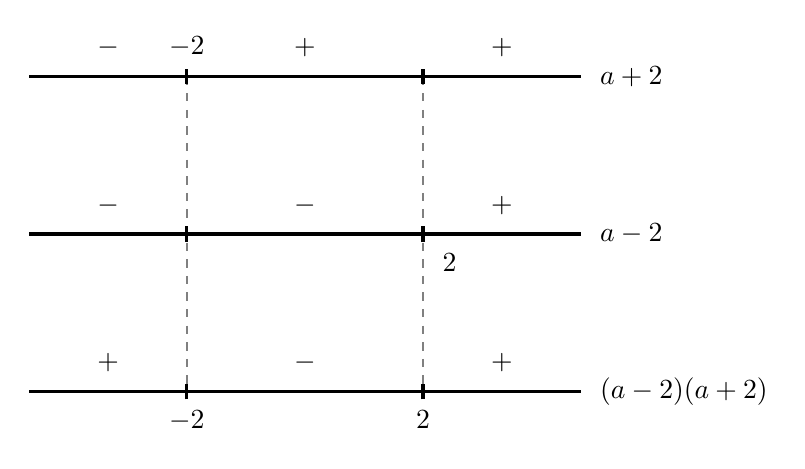
\begin{tikzpicture}
        \node[label=above:{$-2$} ] at (2,6) {};
        \node[label=south east:{2} ] at (5,4) {};
        \node[label=south:{$-2$} ] at (2,2) {};
        \node[label=south:{2} ] at (5,2) {};
        \node[label=east:{$a+2$} ] at (7,6) {};
        \node[label=east:{$a-2$} ] at (7,4) {};
        \node[label=east:{$(a-2)(a+2)$} ] at (7,2) {};
        \node[label=above:{$-$} ] at (1,6) {};
        \node[label=above:{$+$} ] at (3.5,6) {};
        \node[label=above:{$+$} ] at (6,6) {};
        \node[label=above:{$-$} ] at (1,4) {};
        \node[label=above:{$-$} ] at (3.5,4) {};
        \node[label=above:{$+$} ] at (6,4) {};
        \node[label=above:{$+$} ] at (1,2) {};
        \node[label=above:{$-$} ] at (3.5,2) {};
        \node[label=above:{$+$} ] at (6,2) {};
        \draw[very thick] (0, 6) -- (7,6);
        \draw[very thick] (0, 4) -- (7,4);
        \draw[very thick] (0, 2) -- (7,2);
        \draw[gray, thick, dashed] (2, 6) -- (2, 2);
        \draw[gray, thick, dashed] (5, 6) -- (5, 2);
        \draw[very thick] (2, 5.9) -- (2, 6.1);
        \draw[very thick] (5, 5.9) -- (5, 6.1);
        \draw[very thick] (2, 1.9) -- (2, 2.1);
        \draw[very thick] (2, 3.9) -- (2, 4.1);
        \draw[very thick] (5, 3.9) -- (5, 4.1);
        \draw[very thick] (5, 1.9) -- (5, 2.1);
    \end{tikzpicture}
\end{center}

Logo, a expressão é sempre diferente de zero quando $(a-2)(a+2) >0$, ou seja,
quando $a\in(-\infty,-2)\cup(2,+\infty)$.

\bigskip

\textcolor{red}{CHAVE DE PONTUAÇÃO:
    \begin{itemize}
        \item  Identificar que é necessário resolver $\Delta <0$ \emph{(1,0 ponto)};
        \item  Solução da inequação fazendo estudo do sinal da expressão fatorada\emph{(2,0
                  pontos)}.
    \end{itemize} } % Lembrar do "../"
        \end{solution}

        \item \emph{(3{,}0 pontos)} Prove que em todo triângulo a soma dos comprimentos de suas medianas é maior do que seu semiperímetro (metade do perímetro).
           \begin{proof} 
                % Escreva aqui a solução da questão 7.

%\textcolor{red}{ VERSÃO 1 } %Rafaela

Considere o seguinte triângulo de lados $a$, $b$ e $c$, onde $z$, $y$ e $x$ são
suas medianas, respectivamente:

\begin{center}
    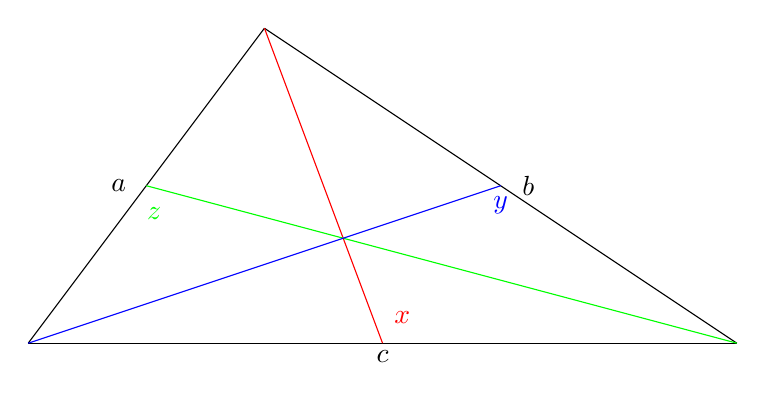
\begin{tikzpicture}
        \draw (0,0) -- (9,0);
        \draw (0,0) -- (3,4);
        \draw (3,4) -- (9,0);
        \node[label=below:{\textbf{$c$}} ] at (4.5,0.15) {};
        \node[label=center:{\textbf{$a$}} ] at (1.15,2) {};
        \node[label=center:{\textbf{$b$}} ] at (6.35,2) {};
        \node[label=below:{\textcolor{red}{\textbf{$x$}}} ] at (4.75,0.65) {};
        \node[label=center:{\textcolor{green}{\textbf{$z$}}} ] at (1.6,1.65) {};
        \node[label=center:{\textcolor{blue}{\textbf{$y$}}} ] at (6,1.75) {};
        \draw[red] (4.5,0) -- (3,4);
        \draw[green] (9,0) -- (1.5,2);
        \draw[blue] (0,0) -- (6,2);
        % \filldraw[red] (1.5,2) circle (0.08);
        % \filldraw[red] (6,2) circle (0.08);
        % \filldraw[red] (4.5,0) circle (0.08);
    \end{tikzpicture}
\end{center}

Queremos provar que: $$x + y + z > \dfrac{a+b+c}{2}.$$ Pela desigualdade
triangular, temos:
\begin{itemize}
    \item  $a < y + \dfrac{b}{2}$ ;
    \item $b < x + \dfrac{c}{2}$;
    \item  $c < z + \dfrac{a}{2}$ .
\end{itemize}
Agora, ``somando'' as desigualdades:
\begin{align*}
    a + b + c < y + x + z + \frac{a}{2} + \frac{b}{2} + \frac{c}{2}
     & \implies a + b + c < y + x + z + \left(\frac{a+b+c}{2}\right) \\
    % & \implies a + b + c - \left(\frac{a+b+c}{2}\right)  < y + x + z + \left(\frac{a+b+c}{2}\right) - \left(\frac{a+b+c}{2}\right)\\
     & \implies \frac{a+b+c}{2} < x+y+z.
\end{align*}
Portanto, provamos que $$x+y+z > \frac{a+b+c}{2}.$$

%\bigskip

%\textcolor{red}{ VERSÃO 2} %autor

%\bigskip

%\textcolor{red}{ VERSÃO 3} % autor

%\bigskip

\bigskip

\textcolor{red}{CHAVE DE PONTUAÇÃO:
    \begin{itemize}
        \item  Uso das 3 desigualdades triangulares \emph{(1,0 ponto)};
        \item Manipulação das inequações \emph{(1,0 ponto)};
        \item  Redação em si (desenho, notação e organização lógica) \emph{(1,0 ponto)}.
    \end{itemize} } % Lembrar do "../"
           \end{proof}

        \item \emph{(3{,}0 pontos)} Sejam $a, b, c \in \R_+^\ast$. Mostre que $$(ab + bc+ ca) \geq a \sqrt{bc} + b \sqrt{ac} + c \sqrt{ab}.$$
           \begin{proof} 
                % Escreva aqui a solução da questão 8.


\textcolor{red}{ VERSÃO 1 } %Rafaela

Sejam $a, b, c \in \R_+^\ast$. Aplicando o Teorema 38 em $a, b \in \R_+^\ast $, teremos:
  \begin{align*}
            \sqrt{ab} \leq \frac{a+b}{2} & \implies c\cdot\sqrt{ab} \leq c\cdot\frac{a+b}{2} &\text{(multiplica por $c>0$)}\\
            & \implies c\sqrt{ab} \leq \frac{ca+cb}{2}, \tag{I} 
\end{align*}       
 em $a, c \in \R_+^\ast $:
 \begin{align*}
            \sqrt{ac} \leq \frac{a+c}{2} & \implies b\cdot\sqrt{ac} \leq b\cdot\frac{a+c}{2} &\text{(multiplica por $b>0$)}\\
                & \implies b\sqrt{ac} \leq \frac{ba+bc}{2}  \tag{II} 
        \end{align*}      
 e em $b, c \in \R_+^\ast $:
 \begin{align*}
            \sqrt{bc} \leq \frac{b+c}{2} & \implies a\cdot\sqrt{bc} \leq a\cdot\frac{b+c}{2} &\text{(multiplica por $a>0$)}\\
                & \implies a\sqrt{bc} \leq \frac{ab+ac}{2}.  \tag{III} 
        \end{align*}
        
``Somando'' (I), (II) e (III), temos:
  \begin{align*}
            c\sqrt{ab} + b\sqrt{ac} + a\sqrt{bc} &\leq \frac{ca+cb}{2} + \frac{ba+bc}{2} + \frac{ab+ac}{2} \\ 
           \implies c\sqrt{ab} + b\sqrt{ac} + a\sqrt{bc} &\leq \frac{2ab+2ac+2bc}{2} \\
           \implies c \sqrt{ab} + b\sqrt{ac} + a\sqrt{bc} &\leq  ab + ac + bc.
        \end{align*}
Portanto, $ ab + ac + bc \geq c\sqrt{ab} + b\sqrt{ac} + a\sqrt{bc}$ para quaisquer $a, b, c \in \R_+^\ast$.






\bigskip


\textcolor{red}{ VERSÃO 2} %Rafaela 

Sejam $a, b, c \in \R_+^\ast$. 

Aplicando o Teorema 38 em $ab, ac \in \R_+^\ast$, teremos:
  \begin{align*}
            \sqrt{ab\cdot ac} \leq \frac{ab+ac}{2} & \implies a\sqrt{bc} \leq \frac{ab+ac}{2}. & \tag{I}
\end{align*}       
Agora em $ba, bc \in \R_+^\ast$, teremos:
  \begin{align*}
            \sqrt{ba\cdot bc} \leq \frac{ba+bc}{2} & \implies b\sqrt{ac} \leq \frac{ba+bc}{2}. & \tag{II}
\end{align*}

Por fim, em $ca, cb \in \R_+^\ast$, teremos:
  \begin{align*}
            \sqrt{ca\cdot cb} \leq \frac{ca+cb}{2} & \implies c\sqrt{ab} \leq \frac{ca+cb}{2}. & \tag{III}
\end{align*}
        
``Somando'' (I), (II) e (III), temos:
  \begin{align*}
            a\sqrt{bc} + b\sqrt{ac} + c\sqrt{ab} &\leq \frac{ab+ac}{2} + \frac{ba+bc}{2} + \frac{ca+cb}{2} \\ 
           \implies a\sqrt{bc} + b\sqrt{ac} + c\sqrt{ab} &\leq \frac{2ab+2ac+2bc}{2} \\
           \implies a\sqrt{bc} + b\sqrt{ac} + c\sqrt{ab} &\leq  ab + ac + bc.
        \end{align*}
Portanto, $ ab + ac + bc \geq c\sqrt{ab} + b\sqrt{ac} + a\sqrt{bc}$ para quaisquer $a, b, c \in \R_+^\ast$.











%\bigskip

%\textcolor{red}{ VERSÃO 3} % autor




%\bigskip





\bigskip

\textcolor{red}{CHAVE DE PONTUAÇÃO:
\begin{itemize}
    \item  Obtenção das 3 desigualdades via Teorema 38 \emph{(1,0 ponto)};
    \item Manipulação das inequações  \emph{(1,0 ponto)};
    \item  Redação em si (desenho, notação e organização lógica) \emph{(1,0 ponto)}.
\end{itemize} } % Lembrar do "../"
           \end{proof}

        \item \emph{(3{,}0 pontos)} Sejam $a, b, c, d \in \R_+^\ast$. Prove que $$\left(a+b+c+d\right) \left( \dfrac 1 a + \dfrac 1 b + \dfrac 1 c + \dfrac 1 d \right) \geq 16.$$
           \begin{proof} 
                % Escreva aqui a solução da questão 9.

\textcolor{red}{ VERSÃO 1 } %Rafaela

Sejam $a, b, c, d \in \R_+^\ast$. Aplicando a desigualdade das médias
aritmética e geométrica nos termos $a , b, c ,d$, temos:
\begin{align*}
    \sqrt[4]{a\cdot b\cdot c\cdot d} \leq \dfrac{a+b+c+d}{4}.\tag{I} \\
\end{align*}

Agora, aplicando a desigualdade das médias harmônica e geométrica nos termos
$a, b, c, d$, temos:
\begin{align*}
    \dfrac{4}{\dfrac{1}{a}+\dfrac{1}{b}+\dfrac{1}{c}+\dfrac{1}{d}} \leq \sqrt[4]{a\cdot b\cdot c\cdot d}. \tag{II}
\end{align*}

Por transitividade de (I) e (II), temos:
\begin{align*}
    %            \dfrac{4}{\dfrac{1}{a}+\dfrac{1}{b}+\dfrac{1}{c}+\dfrac{1}{d}} \leq \sqrt[4]{a\cdot b\cdot c\cdot d} \leq  \dfrac{a+b+c+d}{4} \\
    \dfrac{4}{\dfrac{1}{a}+\dfrac{1}{b}+\dfrac{1}{c}+\dfrac{1}{d}}           & \leq \dfrac{a+b+c+d}{4}                                                                                                                                      \\
    \implies \dfrac{16}{\dfrac{1}{a}+\dfrac{1}{b}+\dfrac{1}{c}+\dfrac{1}{d}} & \leq a+b+c+d                                                                                                                                                 \\
    \implies 16                                                              & \leq (a+b+c+d) \cdot \left(\dfrac{1}{a}+\dfrac{1}{b}+\dfrac{1}{c}+\dfrac{1}{d}\right). & \text{$\left(\dfrac 1 a+\dfrac 1 b+\dfrac 1 c+\dfrac 1 d>0\right)$}
\end{align*}

Portanto, $(a+b+c+d) \cdot
    \left(\dfrac{1}{a}+\dfrac{1}{b}+\dfrac{1}{c}+\dfrac{1}{d}\right) \geq 16$, para
quaisquer $a, b, c, d \in \R_+^\ast$.

%\bigskip

\textcolor{red}{ VERSÃO 2} %Rafaela

Sejam $a, b, c, d \in \R_+^\ast$. Aplicando a desigualdade das médias
aritmética e geométrica nos termos $a , b, c ,d$, temos:
\begin{align*}
    \sqrt[4]{a\cdot b\cdot c\cdot d} \leq \dfrac{a+b+c+d}{4}.\tag{I} \\
\end{align*}

Agora, aplicando a desigualdade das médias harmônica e geométrica nos termos
$a, b, c, d$, temos:
\begin{align*}
    \dfrac{4}{\dfrac{1}{a}+\dfrac{1}{b}+\dfrac{1}{c}+\dfrac{1}{d}} \leq \sqrt[4]{a\cdot b\cdot c\cdot d} & \implies \dfrac{\dfrac{1}{a}+\dfrac{1}{b}+\dfrac{1}{c}+\dfrac{1}{d}}{4} \geq \dfrac{1}{\sqrt[4]{a\cdot b\cdot c\cdot d}}            \\
                                                                                                         & \implies \dfrac{1}{\sqrt[4]{a\cdot b\cdot c\cdot d}} \leq  \dfrac{\dfrac{1}{a}+\dfrac{1}{b}+\dfrac{1}{c}+\dfrac{1}{d}}{4}. \tag{II}
\end{align*}

``Multiplicando'' (I) e (II) (todos os termos são positivos), temos:
\begin{align*}
    \left(\sqrt[4]{a\cdot b\cdot c\cdot d}\right) \cdot \left(\dfrac{1}{\sqrt[4]{a\cdot b\cdot c\cdot d}}\right) & \leq \left(\dfrac{a+b+c+d}{4}\right) \cdot \left(\dfrac{\dfrac{1}{a}+\dfrac{1}{b}+\dfrac{1}{c}+\dfrac{1}{d}}{4}\right) \\
    \implies 1                                                                                                   & \leq \dfrac{(a+b+c+d)\cdot \left(\dfrac{1}{a}+\dfrac{1}{b}+\dfrac{1}{c}+\dfrac{1}{d}\right)}{16}                       \\
    %       \implies 1 \cdot 16 &\leq \dfrac{(a+b+c+d)\cdot \left(\dfrac{1}{a}+\dfrac{1}{b}+\dfrac{1}{c}+\dfrac{1}{d}\right)}{16} \cdot 16 \\
    \implies 16                                                                                                  & \leq (a+b+c+d) \cdot \left(\dfrac{1}{a}+\dfrac{1}{b}+\dfrac{1}{c}+\dfrac{1}{d}\right).
\end{align*}

Portanto, $(a+b+c+d) \cdot
    \left(\dfrac{1}{a}+\dfrac{1}{b}+\dfrac{1}{c}+\dfrac{1}{d}\right) \geq 16$, para
quaisquer $a, b, c, d \in \R_+^\ast$.

%\bigskip

%\textcolor{red}{ VERSÃO 3} % autor

%\bigskip

\bigskip

\textcolor{red}{CHAVE DE PONTUAÇÃO:
    \begin{itemize}
        \item  Obtenção das 2 desigualdades das médias \emph{(1,0 ponto)};
        \item Manipulação das inequações \emph{(1,0 ponto)};
        \item  Redação em si (desenho, notação e organização lógica) \emph{(1,0 ponto)}.
    \end{itemize} } % Lembrar do "../"
           \end{proof}

 
        \end{enumerate}    
\end{document}